% Sistema cilíndrico (ρ,φ,z) con su base (libro fig. 3.2)
\documentclass[border=5pt]{standalone}
\usepackage{tikz}
\usetikzlibrary{arrows.meta, calc}
\begin{document}
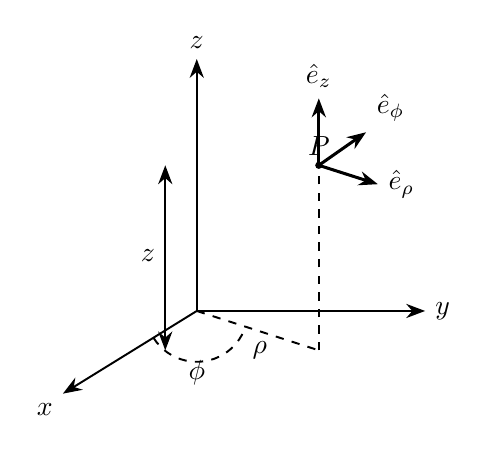
\begin{tikzpicture}[>={Stealth[length=2.4mm]}, line width=0.7pt]
  \coordinate (O) at (0,0);
  \draw[->] (O)--(-1.7,-1.05) node[below left]{$x$};
  \draw[->] (O)--(2.9,0) node[right]{$y$};
  \draw[->] (O)--(0,3.2) node[above]{$z$};
  \coordinate (F) at (1.55,-0.5);   % pie de P en el plano xy
  \coordinate (P) at (1.55,1.85);   % P = F + z
  \draw[dashed] (O)--(F);
  \draw[dashed] (F)--(P);
  \fill (P) circle (1.3pt) node[above]{$P$};
  \node at (0.8,-0.5){$\rho$};
  % ángulo phi (en el plano xy, desde el eje x)
  \draw[dashed] (-0.55,-0.34) arc (212:341:0.65);
  \node at (0.0,-0.78){$\phi$};
  % altura z
  \draw[<->] (-0.4,-0.5)--(-0.4,1.85); \node[left] at (-0.4,0.7){$z$};
  % base en P
  \draw[->, line width=1.1pt] (P)--($(P)+(0,0.85)$) node[above]{$\hat e_z$};
  \draw[->, line width=1.1pt] (P)--($(P)+(0.75,-0.24)$) node[right]{$\hat e_\rho$};
  \draw[->, line width=1.1pt] (P)--($(P)+(0.6,0.42)$) node[above right]{$\hat e_\phi$};
\end{tikzpicture}
\end{document}
